\documentclass[aspectratio=169]{beamer}
\usepackage{amsmath,amssymb,mathtools}
\usepackage{tikz-feynman}
\usepackage{xcolor}
\usepackage{mathrsfs}
\usetheme{metropolis}
\definecolor{graviton}{RGB}{25,60,110}   % deep blue
\definecolor{matter}{RGB}{195,110,30}    % warm orange
\setbeamercolor{alerted text}{fg=graviton}
\usepackage{amsfonts}
\usepackage{braket} % Per una gestione pulita di \Bra, \Ket, \Braket

% Definizione dei colori (adatta i codici esadecimali al tuo tema)
\definecolor{graviton}{RGB}{0, 102, 204}    % Es. Blu per il campo gravitazionale
\definecolor{matter}{RGB}{204, 0, 102}      % Es. Amaranto per la materia
\definecolor{blockbg}{RGB}{245, 247, 250}   % Sfondo leggero per i blocchi

\setbeamercolor{block title}{fg=graviton, bg=blockbg}
\setbeamercolor{block body}{bg=blockbg}
\tikzfeynmanset{
  graviton/.style={photon, thick, color=blue!55!black},
  matter/.style={scalar, thick, color=orange!85!black},
}


\title{Decoherence as a Bridge: From Quantum Foundations to Quantum Future}
\subtitle{Relatori Prof. Angelo Bassi - Doc. Anirudh Gundhi}
\author{Matteo Falasca \\ Fisica Teorica - Curriculum Quantistico, UniTS}
\institute{QFT \quad Quantum Technologies \quad Foundations of QM}
\date{}

\begin{document}
\begin{frame}[plain]
\centering
\vspace{1cm}

\includegraphics[width=0.2\linewidth]{units_sigillo.jpg}\\
{\footnotesize\color{gray} PhD Admission --- Universit\`a di Trieste, Physics}\\[1.3cm]
{\Large Decoherence due to graviton scattering}\\[2pt]
\vspace{0.2cm}
{\small Matteo Falasca}\\[2pt]
{\footnotesize\color{gray} Theoretical Physics - Curriculum: Quantum mechanics\\
Thesis advisors: A.\ Bassi, A.\ Gundhi}
\end{frame}



\begin{frame}[c]
\centering

{\small An \textit{\bfseries\color{graviton}open system} interacting with a
\textit{\bfseries\color{matter}gravitational environment}}\\[0.08cm]
\vspace{0.cm}
{\Large\bfseries\color{graviton!80} What happens to its coherence?$^{[1][2]}$}\\[0.25cm]

\begin{columns}[T,totalwidth=1.05\textwidth]

%---------------- LEFT ----------------
\begin{column}{0.4\textwidth}
\begin{block}{1. Entangled state}
\small

\[
\ket{\Psi(0)} \propto (\ket{S_1}+\ket{S_2})\ket{E_0}
\]

\vspace{-0.7cm}
\[
\Downarrow
\]
\vspace{-1.6cm}

\[
\ket{\Psi(t)} \propto
\ket{S_1}\ket{E_1(t)} +
\ket{S_2}\ket{E_2(t)}
\]

\end{block}
\vspace{3cm}
\end{column}

%---------------- RIGHT ----------------
\begin{column}{0.64\textwidth}
\begin{block}{2. Density matrix}
\small

\[
\hat{\rho}_S(t)=\mathrm{Tr}_E\!\left[\ket{\Psi}\bra{\Psi}\right]\]
\[
\hat{\rho}_S(0)=\frac12
\begin{pmatrix}
1 & 1\\
1 & 1
\end{pmatrix}
\;\longrightarrow\;
\hat{\rho}_S(t)=\frac12
\begin{pmatrix}
1 & \color{matter}{\langle E_2|E_1\rangle}\\
\color{matter}{\langle E_1|E_2\rangle} & 1
\end{pmatrix}
\]

\vspace{-0cm}
\[
\scalebox{1.15}{\boxed{
\color{matter}{\langle E_2(t)|E_1(t)\rangle} \to 0
\;\Longrightarrow\;
\color{graviton}{\text{decoherence}}
}}
\]
\vspace{0.6cm}
%---------------- FIGURE ----------------
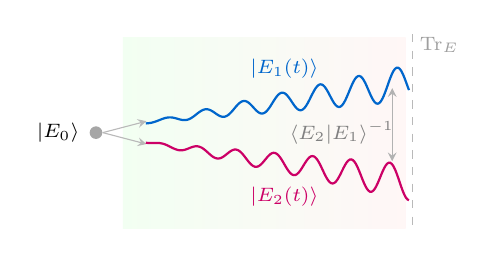
\begin{tikzpicture}[
x=0.9cm,
y=0.85cm,
scale=0.95,
every node/.style={font=\scriptsize},
>=stealth
]

% background
\shade[left color=green!18!white,
       right color=red!12!white,
       opacity=0.28]
(0.4,-1.5) rectangle (4.6,1.5);

%------------------------------------------------
% Initial states
%------------------------------------------------

\fill[gray!70] (0,0) circle (2.4pt);

\node[left,font=\scriptsize] at (-0.1,0)
{$\ket{E_0}$};

% split (stesso punto iniziale, verticale ridotta)
\draw[->,gray!55] (0.10, 0.00) -- (0.75, 0.18);
\draw[->,gray!55] (0.10, 0.00) -- (0.75,-0.18);

%------------------------------------------------
% Environment states
%------------------------------------------------

\draw[graviton,thick,domain=0.74:4.65,samples=170]
plot(\x,
{
0.18
+
(0.021+0.07*(\x-0.9))
*sin(deg(11*(\x-0.9)))
+
0.16*(\x-0.9)
});

\draw[matter,thick,domain=0.74:4.65,samples=170]
plot(\x,
{
-0.18
+
(0.02+0.07*(\x-0.9))
*sin(deg(11*(\x-0.9)+1.2))
-
0.16*(\x-0.9)
});

\node[graviton,above] at (2.8,0.7)
{$\ket{E_1(t)}$};

\node[matter,below] at (2.8,-0.7)
{$\ket{E_2(t)}$};

% overlap

\draw[<->,gray!60] (4.4,0.7)--(4.4,-0.45);

\node[gray] at (3.65,0)
{$\langle E_2|E_1\rangle ^{-1}$};

%------------------------------------------------
% Trace
%------------------------------------------------

\draw[dashed,gray!55] (4.7,1.55)--(4.7,-1.55);

\node[gray!75,above] at (5.1,1.1)
{$\mathrm{Tr}_E$};


\end{tikzpicture}

\end{block}
\end{column}

\end{columns}

\vspace{-0.05cm}

\end{frame}

%---------------------------------------------------------------
%---------------------------------------------------------------
%---------------------------------------------------------------
%---------------------------------------------------------------


\begin{frame}[c]{Linearized Gravity: Free Theory $[3]$}
\vspace{0.4cm}
\begin{columns}[c, totalwidth=\textwidth]

% ══ LEFT ══════════════════════════════════════
\vspace{-0.4cm}
\begin{column}{0.52\textwidth}
{\bfseries\color{graviton}{Metric Expansion:}}
\[
g_{\mu\nu} = \eta_{\mu\nu} + h_{\mu\nu},
\qquad |h_{\mu\nu}|\ll 1
\]

\vspace{0.10cm}

\begin{block}{\small Equation of motion}
\footnotesize
Coordinate invariance:
\(
h_{\mu\nu}\to h_{\mu\nu}+\partial_\mu\xi_\nu+\partial_\nu\xi_\mu
\)\\[4pt]
$\Rightarrow$ Gauge fixing in vacuum leaves only the propagating degrees of freedom of $h_{\mu\nu}$
\end{block}

\vspace{0.15cm}

{\footnotesize Propagating ($\mathrm{TT}$) solutions:
\[
\boxed{
h^{\rm TT}_{ij}(t,z)=
\begin{pmatrix}h_+&h_\times\\h_\times&-h_+\end{pmatrix}
\cos[\omega(t-z/c)]
}\]
\tiny\textcolor{gray!80}{TT: Transverse Traceless}}

\end{column}

% ══ RIGHT: analogies ══════════════════════════
\begin{column}{0.44\textwidth}
\centering

\vspace{0.25cm}

\fbox{%
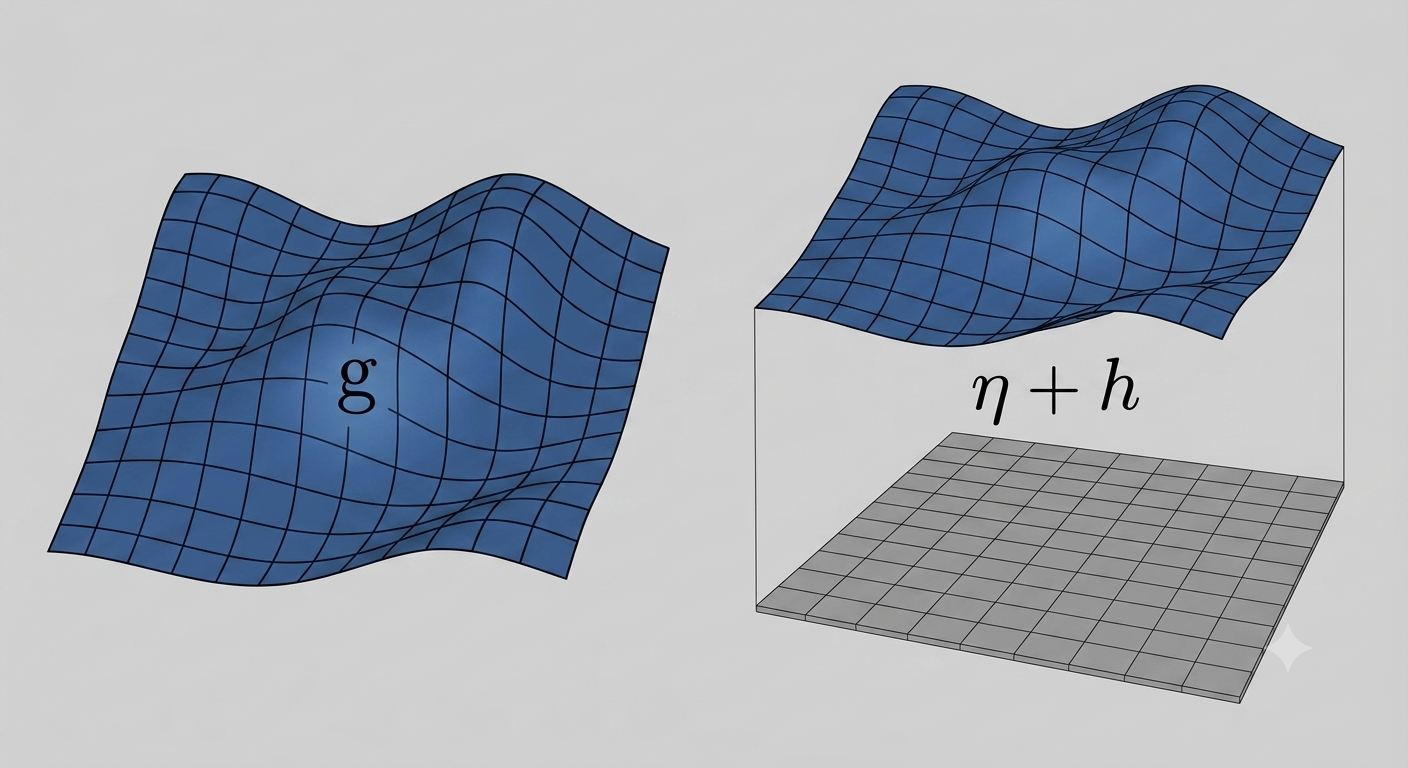
\includegraphics[width=0.88\linewidth]{Decomp.png}
}

\vspace{0.7cm}

{\bfseries\scriptsize\color{matter}
Transverse space-points deformation
}

\vspace{0.00cm}

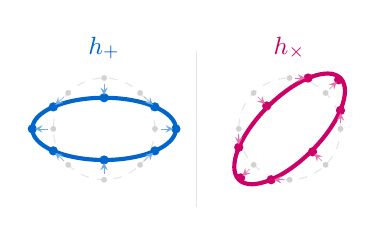
\begin{tikzpicture}[scale=0.76, >=stealth]
    
% h+
\begin{scope}[xshift=-1.55cm]
  \node[graviton, font=\small\bfseries] at (0,1.35) {$h_+$};
  \draw[gray!20,dashed,thin] (0,0) circle (0.85);
  \draw[graviton,line width=1.5pt] (0,0) ellipse (1.20 and 0.52);
  \foreach \ang in {0,45,...,315}{
    \pgfmathsetmacro{\xr}{0.85*cos(\ang)}
    \pgfmathsetmacro{\yr}{0.85*sin(\ang)}
    \pgfmathsetmacro{\xd}{1.20*cos(\ang)}
    \pgfmathsetmacro{\yd}{0.52*sin(\ang)}
    \fill[gray!35] (\xr,\yr) circle (1.4pt);
    \fill[graviton] (\xd,\yd) circle (2.2pt);
    \draw[->,graviton!55,very thin,shorten <=2pt,shorten >=1pt]
      (\xr,\yr)--(\xd,\yd);
  }
\end{scope}

\draw[gray!20,thin] (0,-1.30)--(0,1.30);

% h×
\begin{scope}[xshift=1.55cm]
  \node[matter, font=\small\bfseries] at (0,1.35) {$h_\times$};
  \draw[gray!20,dashed,thin] (0,0) circle (0.85);
  \draw[matter,line width=1.5pt,rotate=45] (0,0) ellipse (1.20 and 0.52);
  \foreach \ang in {0,45,...,315}{
    \pgfmathsetmacro{\xr}{0.85*cos(\ang)}
    \pgfmathsetmacro{\yr}{0.85*sin(\ang)}
    \pgfmathsetmacro{\xd}{0.85*(cos(\ang)+0.363*sin(\ang))}
    \pgfmathsetmacro{\yd}{0.85*(0.363*cos(\ang)+sin(\ang))}
    \fill[gray!35] (\xr,\yr) circle (1.4pt);
    \fill[matter] (\xd,\yd) circle (2.2pt);
    \draw[->,matter!55,very thin,shorten <=2pt,shorten >=1pt]
      (\xr,\yr)--(\xd,\yd);
  }
\end{scope}

\end{tikzpicture}

\end{column}
\end{columns}

\end{frame}


% ---------------- SLIDE 3 ----------------
% ---------------- SLIDE 3 ----------------
% ---------------- SLIDE 3 ----------------
% ---------------- SLIDE 3 ----------------


\begin{frame}{Quantized Linearized Gravity: Interaction with Matter $[4][5]$}

  \small Expand $\sqrt{-g}\mathcal{L}_M$ around flat space, its structure is \textit{analogous to Scalar QED}. 
Split $\mathcal{H} = \mathcal{H}_0 + \mathcal{H}_I$ and quantize:

\[
\mathcal{H}_I =
\underbrace{%
  \tfrac{1}{2}\,\textcolor{graviton}{h_{ij}}\,\partial^i\textcolor{matter}{\phi}\,\partial^j\textcolor{matter}{\phi}
}_{\mathcal{O}(h)}
+
\underbrace{%
  \tfrac{1}{4}\,\textcolor{graviton}{h_{ij}}\textcolor{graviton}{h^{ij}}
  \!\left(\tfrac{1}{2}\partial^\mu\textcolor{matter}{\phi}\partial_\mu\textcolor{matter}{\phi}
         - \tfrac{m^2}{2}\textcolor{matter}{\phi}^2\right)
  + \tfrac{1}{2}\,\textcolor{graviton}{h^{ik}}\textcolor{graviton}{h_k{}^j}\,
    \partial_i\textcolor{matter}{\phi}\,\partial_j\textcolor{matter}{\phi}
}_{\mathcal{O}(h^2)}
\]


\vspace{0.4cm}

The \textbf{scattering amplitude} leading order is $\mathcal{O}(h^2)$:

\begin{center}
\large
\textcolor{graviton}
{$S_{fi}^{(2)} = \bigl\langle\,
  \phi(p'),\, h(k')\,
  \bigm|\,\hat{S}^{(2)}\,\bigm|\,
  \phi(p),\, h(k)
\,\bigr\rangle$\\
}\end{center}


\end{frame}



%-------------------------------------------
%-------------------------------------------
%-------------------------------------------
% =========================================================
% SLIDE 1 -- FROM SCATTERING TO EFFECTIVE DYNAMICS
% =========================================================
\begin{frame}[c]{Matter--Gravity Interactions and Decoherence}

\begin{columns}[c,totalwidth=1.03\textwidth]

%------------------------------------------------
\begin{column}{0.33\textwidth}
\vspace{-0.3cm}
  \centering

{\bfseries Interaction with the gravitational environment}

\vspace{0cm}

\[
\color{graviton}
|S_{fi}^{(2)}|^2 \color{black}=
\left|
\vcenter{\hbox{
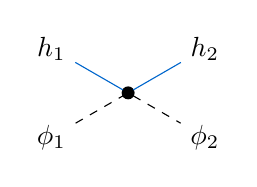
\begin{tikzpicture}[scale=0.75]
\begin{feynman}
  \vertex (i)  at (-1.3,-0.75) {$\phi_1$};
  \vertex (o)  at ( 1.3,-0.75) {$\phi_2$};
  \vertex (v)  at (0,0) [dot] {};
  \vertex (g1) at (-1.3,0.75) {$h_1$};
  \vertex (g2) at ( 1.3,0.75) {$h_2$};
  \diagram*{
    (i)--[scalar](v)--[scalar](o),
    (g1)--[graviton](v),
    (g2)--[graviton](v),
  };
\end{feynman}
\end{tikzpicture}
}}
\right|^2
\]
  

\end{column}

%------------------------------------------------
\begin{column}{0.64\textwidth}

\begin{beamercolorbox}[rounded=true,sep=4pt,center,wd=\linewidth]{block body}
{\bfseries Decoherence}

\[
\hat{\rho}_S(0)=\frac12
\begin{pmatrix}
1 & 1\\
1 & 1
\end{pmatrix}
\;\longrightarrow\;
\hat{\rho}_S(t)=\frac12
\begin{pmatrix}
1 & \color{matter}{\langle E_2|E_1\rangle}\\
\color{matter}{\langle E_1|E_2\rangle} & 1
\end{pmatrix}
\]

\vspace{0.4cm}

\begin{itemize}
\item ${\color{matter}{\rho_{12}(t)}
\propto
\langle E_1(t)|E_2(t)\rangle}$
\end{itemize}

\end{beamercolorbox}

\end{column}

\end{columns}

\vspace{0.6cm}

\begin{center}
{\huge
\[\boxed{
{\color{graviton}
S_{fi}^{(2)}}
\Longrightarrow
{\color{matter}
\rho_{12}(t)}
}\]
}
\end{center}

\end{frame}
%
% =========================================================
% SLIDE
% =========================================================
% =========================================================
% SLIDE -- OUTLOOK: THE ROAD AHEAD
% =========================================================
% =========================================================
% SLIDE -- OUTLOOK: THE ROAD AHEAD
% =========================================================
% =========================================================
% SLIDE -- OUTLOOK: THE ROAD AHEAD
% =========================================================
\begin{frame}{Outlook \& Future Perspectives [2][6][7][8]}
\vspace{0.3cm}

\begin{columns}[T, totalwidth=\textwidth]



% --- COLONNA DESTRA FUSA: Project + Horizon ---
\begin{column}{\textwidth}



\begin{beamercolorbox}[rounded=true, shadow=false, sep=6pt, wd=\linewidth]{block body}
\footnotesize

\textbf{Goal:} Provide state of art framework

\begin{itemize}
    \item Fundamental level analysis
    \item Practical test of \textit{theories of gravity}
\end{itemize}

\vspace{0.2cm}

\textbf{Future Perspectives}

\begin{itemize}
    \item Collapse models $^{[7][8]}$
    \item Modern AMO experiments
\end{itemize}




\end{beamercolorbox}

\end{column}

\end{columns}

\end{frame}

\begin{frame}{References}
\footnotesize

\begin{enumerate}
\item A. Bassi, A. Großardt, H. Ulbricht,
\textit{Gravitational Decoherence},
Class. Quantum Grav. \textbf{34}, 193002 (2017).

\item E. Calzetta, B. L. Hu,
\textit{Nonequilibrium Quantum Field Theory},
Cambridge University Press (2008).

\item M. Maggiore,
\textit{Gravitational Waves, Vol. I: Theory and Experiments},
Oxford University Press (2008).

\item W. Greiner, J. Reinhardt,
\textit{Quantum Electrodynamics},
Springer (2009).

\item W. Greiner, J. Reinhardt,
\textit{Field Quantization},
Springer (1996).

\item A. Gundhi, A. Bassi,
\textit{Motion of an Electron through Vacuum Fluctuations},
Phys. Rev. A \textbf{108}, 012212 (2023).


\item A. Bassi, K. Lochan, S. Satin, T. P. Singh, H. Ulbricht,
\textit{Models of Wave-Function Collapse, Underlying Theories, and Experimental Tests},
Rev. Mod. Phys. \textbf{85}, 471 (2013).

\item M. Toroš, A. Bassi,
\textit{Bounds on Collapse Models from Matter-Wave Interferometry},
J. Phys. A: Math. Theor. \textbf{51}, 115302 (2018).
\end{enumerate}

\end{frame}


% --- SLIDE DI RINGRAZIAMENTO ---
\begin{frame}[plain, c]
    \centering
    \vspace{0.5cm}
    {\Huge \bfseries \color{graviton} Thank you for your attention}
    
    \vspace{1cm}
    \begin{columns}[c]
        \begin{column}{0.5\textwidth}
            \centering
            \footnotesize \color{gray}
            \textbf{Matteo Falasca}\\
            \texttt{Prof. Angelo Bassi}\\
            \texttt{Doc. Anirudh Ghundi}\\
            University of Trieste \\ Theoretical Physics
        \end{column}
        \begin{column}{0.5\textwidth}
          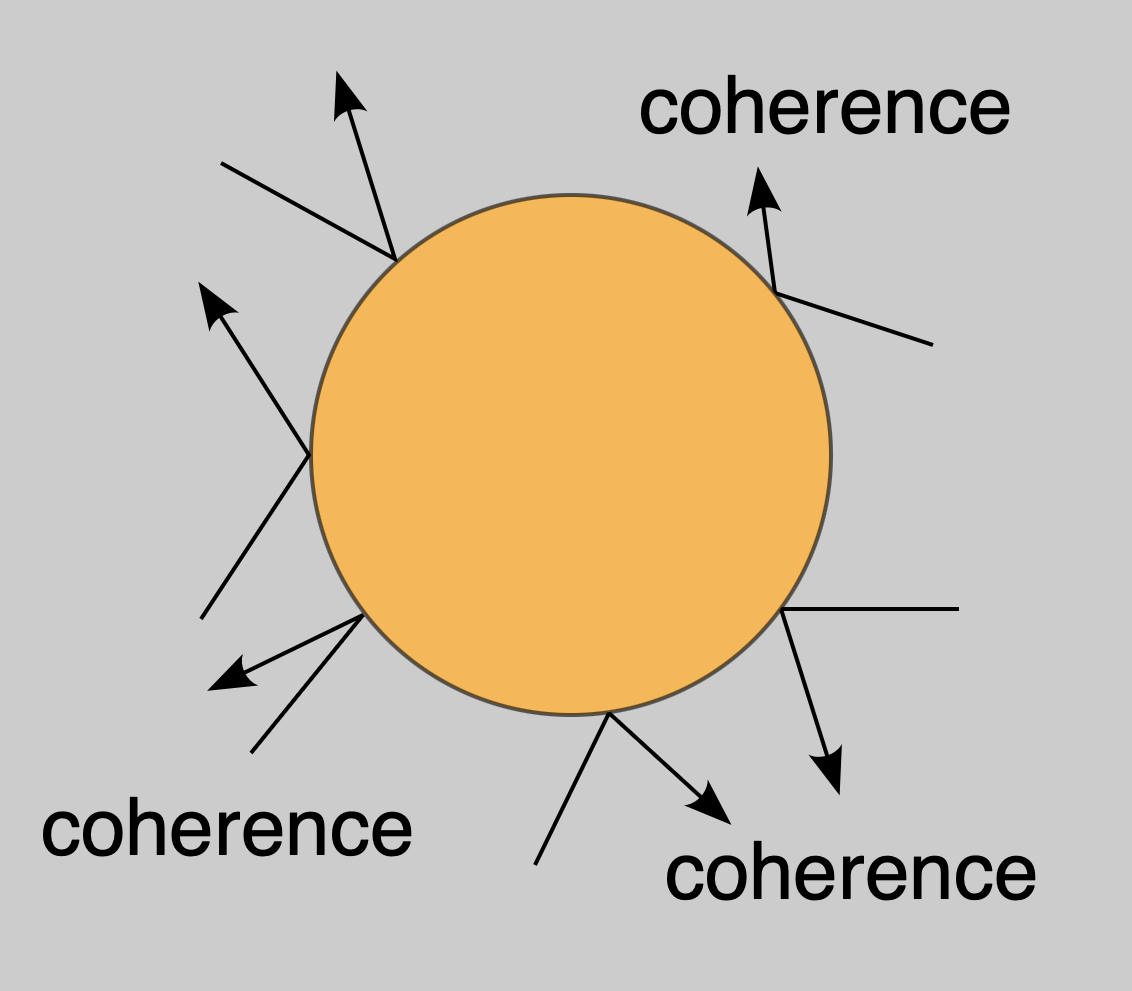
\includegraphics[width=5cm]{Screenshot 2026-06-20 alle 13.34.29.png}  
        \end{column}    
    \end{columns}
\end{frame}


\definecolor{graviton}{RGB}{0,102,204}
\definecolor{matter}{RGB}{204,0,102}
\definecolor{blockbg}{RGB}{245,247,250}
 
\setbeamercolor{alerted text}{fg=graviton}
\setbeamercolor{block title}{fg=graviton, bg=blockbg}
\setbeamercolor{block body}{bg=blockbg}
 
% ── convenience macros ──────────────────────────────────────────
\newcommand{\grav}[1]{\textcolor{graviton}{#1}}
\newcommand{\matt}[1]{\textcolor{matter}{#1}}
\newcommand{\half}{\tfrac{1}{2}}
 
% ================================================================
%  BACKUP 1 — INTERACTION FROM MATTER ACTION
% ================================================================
\begin{frame}[c]{Backup 1 — Graviton–Matter Interaction from $S_M$}
 
\small
Expand $S_M = \int d^4x\,\sqrt{-g}\,\mathcal{L}_M[\phi,g_{\mu\nu}]$
around $g_{\mu\nu}=\eta_{\mu\nu}+h_{\mu\nu}$.
 
\vspace{0.15cm}
 
\begin{columns}[T, totalwidth=\textwidth]
 
% ── LEFT ────────────────────────────────────────────────────────
\begin{column}{0.48\textwidth}
 
\begin{block}{Metric expansion to $\mathcal{O}(h^2)$}
\footnotesize
\[
g^{\mu\nu}
= \eta^{\mu\nu}-h^{\mu\nu}+h^\mu_{\ \alpha}h^{\alpha\nu}
\]
\[
\sqrt{-g}
= 1+\tfrac{h}{2}+\tfrac{1}{4}\!\left(\tfrac{h^2}{2}-h_{\alpha\beta}h^{\alpha\beta}\right)
\]
From $g^{\mu\alpha}g_{\alpha\beta}=\delta^\mu_\beta$ and
$\ln\det(-g)=\mathrm{tr}\ln(-g)$.
\end{block}
 
\vspace{0.2cm}
 
\begin{block}{Free term}
\footnotesize
\[
S_M^{(0)}=\int d^4x
\!\left(\half\eta^{\mu\nu}\partial_\mu\phi\,\partial_\nu\phi
-\tfrac{m^2}{2}\phi^2\right)
\]
\end{block}
 
\end{column}
 
% ── RIGHT ───────────────────────────────────────────────────────
\begin{column}{0.52\textwidth}
 
\begin{block}{Linear vertex — couples $h$ to $T_{\mu\nu}$}
\footnotesize
\[
S_M^{(1)}=-\half\int d^4x\;
\grav{h^{\mu\nu}}T_{\mu\nu}
\]
\[
T_{\mu\nu}=\partial_\mu\matt{\phi}\,\partial_\nu\matt{\phi}
-\eta_{\mu\nu}\!\left(\half\partial_\rho\matt{\phi}\,\partial^\rho\matt{\phi}
+\tfrac{m^2}{2}\matt{\phi}^2\right)
\]
\end{block}
 
\vspace{0.2cm}
 
\begin{block}{Seagull vertex — two graviton legs}
\footnotesize
\begin{align*}
S_M^{(2)}=\int d^4x\Bigl[&
\tfrac{1}{4}\!\left(\tfrac{h^2}{2}-h_{\alpha\beta}h^{\alpha\beta}\right)\mathcal{L}_M\\
&-\tfrac{h\,h^{\mu\nu}}{4}\partial_\mu\matt{\phi}\,\partial_\nu\matt{\phi}
+\half\grav{h^{\mu\alpha}h_\alpha^{\ \nu}}\partial_\mu\matt{\phi}\,\partial_\nu\matt{\phi}
\Bigr]
\end{align*}
In TT gauge ($h^{0\mu}=0$): time components vanish.
\end{block}
 
\end{column}
\end{columns}
 
\end{frame}
 
% ================================================================
%  BACKUP 2 — CANONICAL QUANTIZATION
% ================================================================
\begin{frame}[c]{Backup 2 — Canonical Quantization of the Graviton}
 
\begin{columns}[T,totalwidth=\textwidth]
 
% ── LEFT ────────────────────────────────────────────────────────
\begin{column}{0.51\textwidth}
 
\begin{block}{Mode expansion}
\footnotesize
\[
\grav{\hat{h}_{\mu\nu}}(x)=\int\!\frac{d^3k}{\sqrt{(2\pi)^3 2\omega_k}}
\sum_{\lambda=+,\times}
\!\Bigl(\hat{a}_{\vec{k},\lambda}\,e^{-ik\cdot x}\,\epsilon_{\mu\nu}^{(\lambda)}
+\mathrm{h.c.}\Bigr)
\]
\end{block}
 
 
\begin{block}{Polarization tensors}
\footnotesize
\[
\epsilon^{(+)}_{\mu\nu}=\tfrac{1}{\sqrt{2}}(u_\mu u_\nu - v_\mu v_\nu)
\]
\[
\epsilon^{(\times)}_{\mu\nu}=\tfrac{1}{\sqrt{2}}(u_\mu v_\nu + v_\mu u_\nu)
\]
$\{u,v,n\}$ orthonormal; $n$ = propagation direction.
\end{block}
 
 \vspace{-0.1cm}
\begin{block}{TT projector}
\footnotesize
\[
\Lambda_{ij,kl}=\sum_\lambda\epsilon^{(\lambda)}_{ij}\epsilon^{(\lambda)}_{kl}
=\half\!\left(P_{ik}P_{jl}+P_{il}P_{jk}-P_{ij}P_{kl}\right)
\]
with $P_{ij}=\delta_{ij}-n_i n_j$.
\end{block}
 
\end{column}
 
% ── RIGHT ───────────────────────────────────────────────────────
\begin{column}{0.50\textwidth}
 
\begin{block}{ETCR $\to$ oscillator algebra}
\footnotesize
Impose:
\[
\bigl[\hat{h}_{\mu\nu}(\vec{x},t),\,\hat{\pi}_{\alpha\beta}(\vec{x}',t)\bigr]
=i\,\delta^{(3)}(\vec{x}-\vec{x}')\,\delta^{\mu\nu}_{\ \,\alpha\beta}
\]
\vspace{-0.2cm}
Invert via the covariant product
\[
\langle A,B\rangle = i\!\int d^3x\;
A^{*}_{\mu\nu}\overset{\leftrightarrow}{\partial_0}B^{\mu\nu}
\]
to get $\hat{a}_{\vec{k},\lambda}=\langle h(\vec{k},\lambda),\hat{h}\rangle$,
then compute the commutator:
\[
\boxed{
\bigl[\hat{a}_{\vec{k},\lambda},\,\hat{a}^\dagger_{\vec{k}',\lambda'}\bigr]
=\delta^{\lambda}_{\ \lambda'}\,\delta^{(3)}(\vec{k}-\vec{k}')
}
\]
\end{block}
 

 
\end{column}
\end{columns}
 
\end{frame}
 
% ================================================================
%  BACKUP 3 — SEAGULL AMPLITUDE
% ================================================================
\begin{frame}[c]{Backup 3 — Seagull Scattering Amplitude}

\small
Process: $\matt{\phi}(k_3)+\grav{h}(k_4,\lambda_4)\to\matt{\phi}(k_1)+\grav{h}(k_2,\lambda_2)$,
contact term from $\hat{S}^{(1)}$ at $\mathcal{O}(\kappa^2)$.

\vspace{0.2cm}

\begin{columns}[T,totalwidth=\textwidth]

% ── LEFT ─────────────────────────────────────────
\begin{column}{0.5\textwidth}

\begin{block}{Vertices ($\mathcal{O}(\kappa^2)$)}
\footnotesize
\[
V_1=-\tfrac{1}{8}h_{\alpha\beta}h^{\alpha\beta}
\big[(\partial^*\phi)^2-m^2\phi^2\big]\]\[
V_2=\tfrac12 h^{\mu\alpha}h_\alpha^{\ \nu}\partial_\mu\phi\,\partial_\nu\phi
\]
\end{block}

\vspace{0.2cm}

\begin{block}{Mode expansion}
\footnotesize
Select terms with
$\hat{a}_{k_2,\lambda_2}\hat{a}_{k_4,\lambda_4}$ and
$\hat{a}^\dagger_{k_1}\hat{a}_{k_3}$.

\end{block}

\end{column}

% ── RIGHT ────────────────────────────────────────
\begin{column}{0.5\textwidth}

\begin{block}{Momentum conservation}
\footnotesize
\[
\int d^4x\,e^{i(K_{\rm out}-K_{\rm in})x}
=(2\pi)^4\delta^{(4)}(\Delta K)
\]
\end{block}

\vspace{-0.2cm}
\begin{block}{Tensor structure}
\footnotesize
\[
V_1:\ (\epsilon_2\!\cdot\!\epsilon_4)(-k_1\!\cdot\!k_3+m^2),
\quad
V_2:\ \epsilon_{2}^{\mu\alpha}\epsilon_{4\alpha}^{\ \nu}k_{1\nu}k_{3\mu}
\]
\[
\epsilon(k_2,+)\cdot \epsilon(k_4,+)=\frac12(1+\cos^2\theta),\quad\]\[
\epsilon(k_2,\times)\cdot \epsilon(k_4,\times)=\cos\theta\quad \text{$\theta$ = scattering angle}
\]
\end{block}

\end{column}
\end{columns}

\vspace{0.0cm}

\begin{beamercolorbox}[rounded=true,sep=4pt,wd=\linewidth]{block body}
\footnotesize
\[
S_{fi}^{\rm seagull}
=
\frac{i\,\delta^{(4)}(\Delta K)}{(2\pi)^2\sqrt{16E_1E_2E_3E_4}}
\Big[
\tfrac12(\epsilon_2\!\cdot\!\epsilon_4)(-k_1\!\cdot\!k_3+m^2)
+\epsilon_{2}^{\mu\alpha}\epsilon_{4\alpha}^{\ \nu}k_{1\nu}k_{3\mu}
\Big]
\]
\end{beamercolorbox}

\end{frame}

%--------------------------
%--------------------------
%--------------------------
%--------------------------
%--------------------------
\end{document}

